\chapter{Data}
\label{ch:data}

We drew on two datasets, one from the Proto0 DarkSide test prototype at CERN,
and one from the Laboratori Nazionali del Gran Sasso (LNGS) cryogenic setup.
We did not collect new data for this thesis.

Both datasets contain digital traces of photodetector modules (PDMs) output,
divided in continuous chunks of fixed length that we call ``events''.
Optionally, a pulsed laser is shone at the detector and the temporal window
of the event waveform is synchronized with the laser.

\section{Proto0}

Proto0 is a small test time projection chamber (TPC) in liquid argon (LAr)
built and operated in CERN building 182 between 2019 and 2020, now to be
operated again in Napoli in 2021. The CERN wiki page is
\url{https://twiki.cern.ch/twiki/bin/view/Sandbox/DarkSideProto0} (unrestricted
access). Note that the descriptions in \cite[sec.~4.3.2]{luzzi2020} and in the
Yellow Book \cite[65]{aalseth2018} contain outdated information relative to the
status of the setup when the data we are considering was recorded.

The TPC size is $\SI{30}{cm} \times \SI{30}{cm} \times \SI{20}{cm}$. On top of
the TPC sits a photodetector unit (PDU), i.e.\ data transmission electronics
plus a motherboard, this specific one officiously dubbed ``Motherboard 2''
(MB2), consisting in a matrix of $5\times 5$ PDMs. The silicon photomultipliers
(SiPMs) Tiles mounted in the PDMs were fabricated by Fondazione Bruno Kessler
(FBK) in 2019, and are all triple doped. The tiling scheme of the motherboard
is shown in \autoref{fig:pdmadcch}, while in \autoref{fig:proto0} there are
some photos of the apparatus.

The PDM outputs are each sent to an analog to digital converter (ADC) channel.
The ADC has depth \SI{16}{bit} and sampling frequency \SI{125}{MSa/s}, the same
specifics which will be adopted in DarkSide20k.

Of the Proto0 data, we used only a ``baseline'' acquisition, i.e.\ with the
PDMs biased below breakdown voltage and thus insensitive to light. So the
waveforms contain only electrical noise. This data file is not publicly
available. There are 1000~events, each \SI{0.5}{ms} long.

In \autoref{fig:hist2dtile64} we show a two-dimensional histogram of the events
for Tile~64 as an example. The variables are the sample number in the event and
the ADC value. It is like stacking on each other all the waveforms. This kind
of visualization is also called ``persistence plot''. In
\autoref{tab:proto0meta} we list for reference the metadata of the
acquisition, linked on the CERN wiki.

\begin{figure}
    
    \widecenter{
        \newlength\protoheight
        \setlength\protoheight{7.5cm}
        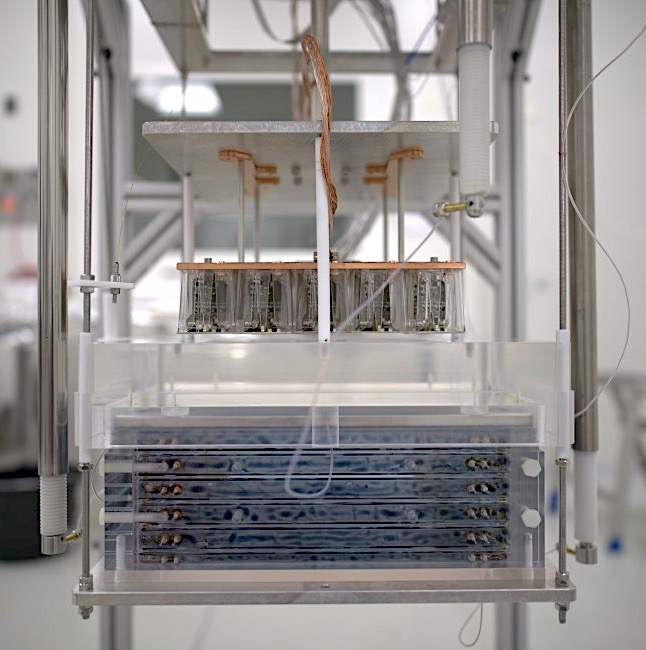
\includegraphics[height=\protoheight]{proto0-1}
        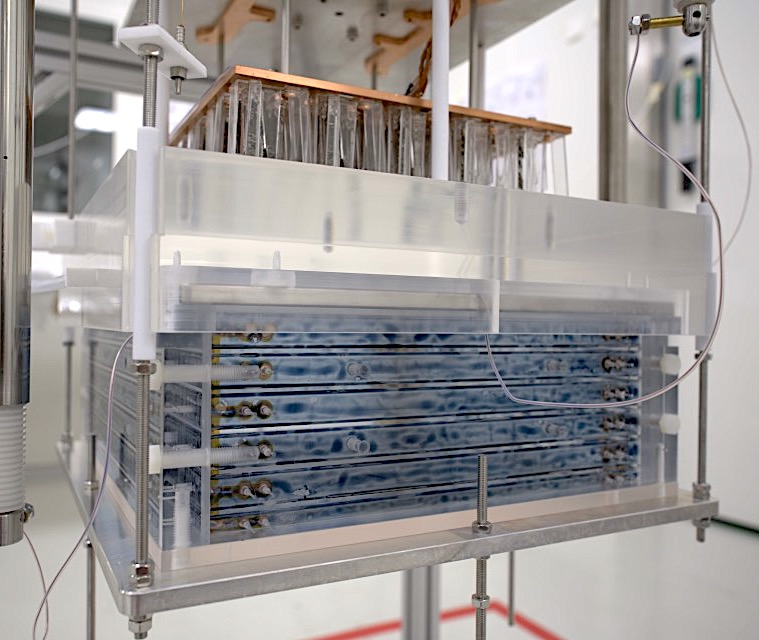
\includegraphics[height=\protoheight]{proto0-2}
    }
    
    \caption{\label{fig:proto0} The Proto0 TPC outside of the cryostat, from
    \cite[50]{luzzi2020}. When in the cryostat, the whole object is completely
    submerged in LAr. Inside the bluish box there is a uniform electric field
    pointing top to bottom. The stripes on the sides are conductive and are the
    steps of a voltage divider, to create boundary conditions that keep the
    field uniform even near the borders. The metal frame visible just over the
    blue box, behind the semitransparent plastic, is the support of the grid
    used to create an high field region above it up to the anode. That region
    is contained in a ``gas pocket'', i.e.\ something like a cup kept
    upside-down underwater. The pocket is kept filled with gaseous argon. The
    copper frame on the top supports the PDMs, with their characteristic
    plastic case holding the front end board (FEB) attached orthogonally to the
    SiPMs Tile.}
    
\end{figure}

\begin{figure}
    
    \widecenter{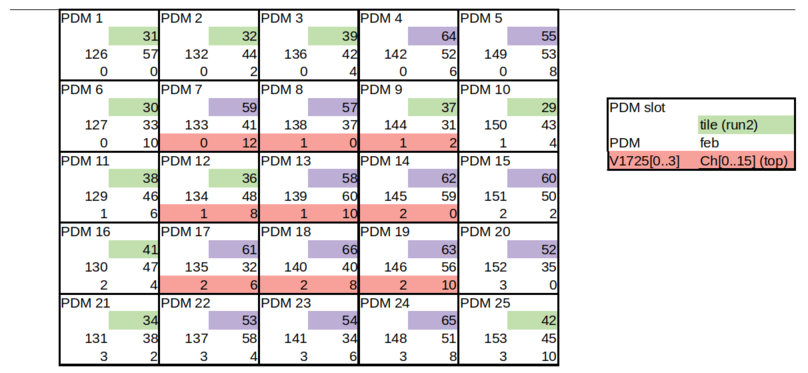
\includegraphics[width=1.2\textwidth]{PDMadcCh}}
    
    \caption{\label{fig:pdmadcch} Schematic of the motherboard installed in
    Proto0, showing the SiPM Tile identification number of each PDM and the ADC
    channels. The color of the Tile number sets apart the two set of SiPMs
    used: green ``run2'' have a higher breakdown voltage than violet ``run4'';
    being all operated at the same bias, the run2 Tiles have overvoltage
    \SI{5.5}{V} while run4 \SI{6.5}{V}. The PDMs marked in red are the inputs
    of the data trigger, which is not used in the data we consider.}

\end{figure}

% info on Proto0:
% Report_v1 Report on DAQ operation of MB1 test setup at CERN.pdf, page 1 and 2
% Kish_DS_CollabMeeting-Nov2019_Naples_Proto0 DarkSide Proto-0 activities.pdf
% Darkside_general_meeting_Napoli_Last updates on the tests and the next steps toward DS Proto 1ton.pdf, pages 12--18

\clearpage
\section{LNGS}
\label{sec:lngsdata}

\newcommand\lngsport{2180}
\newcommand\lngsbase{http://ds50tb.lngs.infn.it:\lngsport/SiPM/Tiles}

At LNGS there is a testing setup for individual SiPMs or Tiles. Briefly
described in the Yellow Book \cite[34]{aalseth2018}, it is presented in great
detail in \cite{acerbi2017} and \cite[ch.~3]{savarese2018}. However in these
references the data acquisition process is evidently different from the one
used for the data at hand, where a laser is employed. We do not know the
specifics of the laser. We presume that apart from the laser the rest of the
equipment stayed the same, and that the preamplifier used is the one included
in the stand instead of the FEB of the PDM.

The dataset we are considering was collected between the end of 2020 and
beginning of 2021 by Lucia Consiglio. It contains all the FBK Tiles used in
Proto0 apart from Tile~55, plus other newer Tiles produced by LFoundry,
Tiles~15, 21, 22, and~23. The data is publicly available in the directories
\url{\lngsbase/FBK/NUV/MB2-LF-3x/} and
\url{\lngsbase/LFOUNDRY/pre-production-test/}. The directory name
\texttt{MB2-LF-3x} stands for ``Motherboard 2, low field, triple doping''.

The events are laser-triggered and recorded in \texttt{wav} files. Each file
contains one to three channels; one channel is the Tile output, another is the
recorded laser trigger channel, containing a square pulse marking the trigger
location, which occurs at the same place relative to the event start varying in
a \SI{23}{ns} range (see \autoref{fig:triggerhist}), and the third contains
some kind of signal we do not understand and did not investigate. Files with
one channel have only the PDM channel, those with two have the PDM and the
laser trigger. Of the two-channels files we used, the channel layout is 0:PDM,
1:trigger for FBK, swapped for LFoundry.

The layout of the \texttt{wav} files is the following. The files are arrays of
16~bit signed integers, divided into events. Each event starts with 20 values
of metadata, followed by \num{15001} values for each channel. The values in the
metadata are: 0:~the constant $-1$, 1:~the length of the metadata, i.e.\ 20,
6:~the length of the event, i.e.\ \num{15001}, 10:~the number of channels,
i.e.\ 1, 2 or~3. We inferred this layout from the files we looked at, some
details may be different for other files. The ADC has depth 10~bit, so the
values are always in the range 0 to~1023. The sampling frequency is
\SI{1}{GSa/s}.

In \autoref{fig:hist2dtile64} we show the persistence plot for the particularly
noisy Tile~52, synchronized with the laser trigger. The discretized height of
pulses is well visible, and there also some random pulses arriving before the
trigger. The response of the SiPM will be described briefly in \autoref{ch:snr}
and more in detail in \autoref{ch:anal}.

\begin{table}
    
    \widecenter{
        \begin{tabular}{llll}
            \toprule
            Field                 & Value        & Field                        & Value            \\
            \cmidrule(r){1-2}                    \cmidrule(l){3-4}              
            run                   & 886          & gas pocket                   & ON               \\
            date(dd-mm)           & 5-11         & laser intensity              &                  \\
            run type              & baseline run & trigger                      & external (50 Hz) \\
            Quality               & good         & trigtime (\si{\micro s})     & 100              \\
            Problem               &              & post-trigger (\si{\micro s}) & 400              \\
            Nevents (k)           &              & Time gate  (\si{\micro s})   & 500              \\
            Edrift (V/cm)         & 200          & PDM Coindidence              &                  \\
            Eextraction (kV/cm)   & 2.8          & Threshold extent (ns)        & 80               \\
            SiPM tension (V)      & 50           & TPC pressure (mbarg)         & >450             \\
            \bottomrule
        \end{tabular}
    }
    
    \caption{\label{tab:proto0meta} Metadata for the Proto0 baseline run~886.}
    
\end{table}

\begin{figure}
    
    \widecenter{\includempl{fighist2dtile64}}
    
    \figcaption{hist2dtile64}{Time-value histogram of the waveforms for Tile~64
    in the Proto0 data.}
    
\end{figure}

\begin{figure}
    
    \widecenter{\includempl{fighist2dtile52}}
    
    \figcaption{hist2dtile52}{Time-value histogram of the waveforms for Tile~52
    in the LNGS data.}
    
\end{figure}

\marginpar{Add a raw zoomed plot of the Proto0 noise waveform.}
